\documentclass[a4paper,12pt]{article}
\usepackage[fleqn]{amsmath}
\usepackage{amssymb}
\usepackage{graphicx}
\graphicspath{ {./images/} }
\begin{document}

\title{Trigonometry}	
\author{Edward Jex}
\maketitle
\section*{The Radian}
$\pi$ radians $= 180$ degrees \\ 
\subsection*{Arc length}
\begin{align*}
l & = \frac{\theta 2 \pi r}{2 \pi} \\
& = r \theta \\
\end{align*}
\subsection*{Sector area} 
\begin{align*}
A & = \frac{\theta}{2 \pi} \pi r^2 \\
& = \frac{r^2 \theta}{2} \\
\end{align*}
\section*{Trigonometry}
Values of $\sin$, $\cos$ and $\tan$ can be worked out by using triangles.

\begin{center}
\begin{tabular}{ c | c c c c c }
\hline
	 & $0$ & $\frac{\pi}{6}$ & $\frac{\pi}{4}$ & $\frac{\pi}{4}$ & $\frac{\pi}{2}$ \\ 
\hline
	$\sin \theta$ & $0$ & $\frac{1}{2}$ & $\frac{1}{\sqrt{2}}$ & $\frac{\sqrt{3}}{2}$ & $1$ \\ 
	$\cos \theta$ & $1$ & $\frac{\sqrt{3}}{2}$ & $\frac{1}{\sqrt{2}}$ & $\frac{1}{2}$ & $0$ \\ 
	$\tan \theta$ & $0$ & $\frac{1}{\sqrt{3}}$ & $1$ & $\sqrt{3}$ & NaN \\ 
\hline
\end{tabular}
\end{center}
\subsection*{The unit circle}
\subparagraph*{Identities}
\begin{align*}
\tan \theta & \equiv \frac{\sin \theta}{\cos \theta} \\
\sin^2 \theta + \cos^2 \theta & \equiv 1 \\
\end{align*}
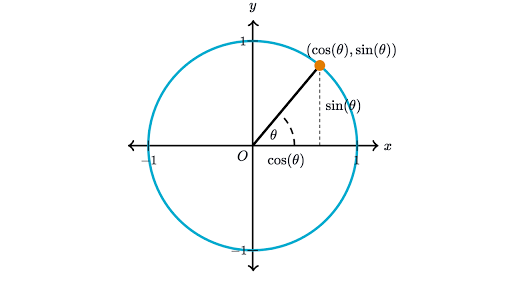
\includegraphics[scale=0.7]{UnitCircle} \\\\
$\sin$ and $\cos$ graphs have a period of $2\pi$, $\tan$ has a period of $\pi$. \\
$\sin$ and $\tan$ have a rotational symmetry about the origin. \\
$\cos$ has a line of symmetry on the y axis \\
\begin{align*}
\cos - \theta & = \cos \theta \\
\sin - \theta & = - \sin \theta \\
\tan - \theta & = - \tan \theta \\ 
\end{align*}
\section*{Solving Equations}
Be careful not to divide by an expression that may be 0 as you may lose solutions. Also note that there may be many solutions in a given range. Drawing a CAST diagram or graph sketch may be useful.
\subsection*{Example 1}
\begin{align*}
\text{Solve} \sin \theta - 2 \cos \theta & = 0 \hspace*{1cm} \text{for } 0 \leqslant \theta < 2\pi \\
\sin \theta & = 2 \cos \theta \\
\frac{\sin \theta}{\cos \theta} & = 2 \\
\tan \theta & = 2 \\
\theta & = \arctan 2 \\
\theta & = 1.107, 4.249 \\
\end{align*}
Note, two solutions.
\subsection*{Example 2}
\begin{align*}
\text{Solve } 2 \cos \theta \sin \theta & = \cos \theta \hspace*{1cm} \text{for } 0 \leqslant \theta <  2\pi \\
2 \cos \theta \sin \theta - \cos \theta & = 0 \\
\cos \theta (2\sin \theta - 1) & = 0 \\
\cos \theta = 0 \hspace*{1cm} & \hspace*{1cm} \sin \theta = \frac{1}{2} \\ 
\theta & = \frac{\pi}{6}, \frac{\pi}{4}, \frac{5 \pi}{6}, \frac{3 \pi}{2} \\
\end{align*}
\subsection*{Example 3}
\begin{align*}
\text{Solve } \sin^2 \theta + \sin \theta & = \cos^2 \theta \hspace*{1cm} \text{for } 0 \leqslant \theta < 2 \pi \\
\sin^2 \theta + \sin \theta & = 1 - \sin^2 \theta \\
2 \sin^2 \theta + \sin \theta & = 1 \\
2 \sin^2 \theta + sin \theta - 1 & = 0 \\
(\sin \theta + 1)(2 \sin \theta -1) & = 0 \\
\sin \theta = -1 \hspace*{1cm} & \hspace*{1cm} \sin \theta = \frac{1}{2} \\
\theta = \frac{\pi}{6}, \frac{5 \pi}{6}, \frac{3 \pi}{2} & \\ 
\end{align*}
\section*{Sine and Cosine rules}
\begin{align*}
\frac{\sin A}{a} & = \frac{\sin B}{b} = \frac{\sin C}{c} \\
a^2 &= b^2 + c^2 - 2bc \cos A \\ 
\end{align*}
Area of a triangle $ = \frac{1}{2} ab \sin C$ \\ 
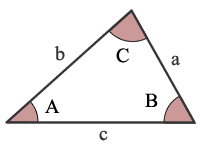
\includegraphics[scale=0.7]{Triangle} \\\\
\section*{Small Angle Approximations}
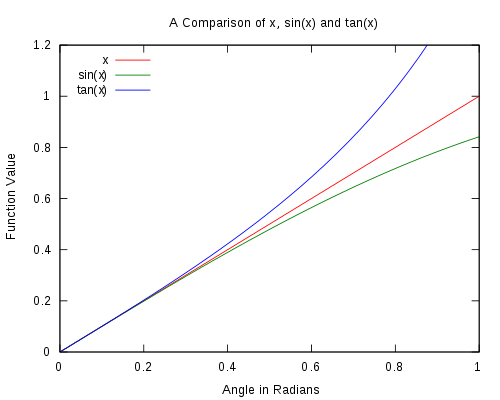
\includegraphics[scale=0.5]{Graph1} \\
At small angles, trigonometric functions can be approximated. For small $\theta$:
\begin{itemize}
	\item $\sin \theta \simeq \theta$
	\item $\tan \theta \simeq \theta$
	\item $\cos \theta \simeq 1 - \frac{\theta^2}{2}$
\end{itemize}
These approximations can be found in the first few terms of the Taylor series expansions of the trigonometric functions. They can be used to more easily solve functions with small angles. 
\section*{Further Trig Functions}
The reciprocals of trig functions have their own notations. \\
\begin{tabular}{ c c }
\hline
	 $f(x)$ & $\frac{1}{f(x)}$  \\ 
\hline
	$\sin x$ & $\csc x$ \\
	$\cos x$ & $\sec x$ \\
	$\tan x$ & $\cot x$ \\
\hline
\end{tabular}
\end{document}